\documentclass[UTF8,a4paper,11pt]{ctexart}

% ============================================================
% PulseArena Technical Report -- polished manuscript
% ============================================================

\usepackage[margin=1in,headheight=15pt]{geometry}
\usepackage{amsmath,amssymb,mathtools,bm}
\usepackage{booktabs,tabularx,array}
\usepackage{graphicx}
\usepackage{xcolor}
\usepackage{hyperref}
\usepackage{tikz}
\usepackage{pgfplots}
\usepackage{listings}
\usepackage{fancyhdr}
\usepackage{titlesec}
\usepackage{float}
\usepackage{caption}
\usepackage{enumitem}
\usepackage{microtype}

\usetikzlibrary{
    arrows.meta,
    positioning,
    calc,
    backgrounds,
    fit,
    matrix,
    shapes.geometric
}
\pgfplotsset{compat=1.18}

% -------------------- Color system --------------------
\definecolor{paBlue}{HTML}{315C9B}
\definecolor{paLightBlue}{HTML}{EEF4FB}
\definecolor{paTeal}{HTML}{2A8C82}
\definecolor{paLightTeal}{HTML}{EFF8F6}
\definecolor{paOrange}{HTML}{C87932}
\definecolor{paLightOrange}{HTML}{FCF4EC}
\definecolor{paRed}{HTML}{B94B4B}
\definecolor{paGray}{HTML}{5C6673}
\definecolor{paLightGray}{HTML}{F4F6F8}
\definecolor{codegreen}{rgb}{0,0.48,0}
\definecolor{codegray}{rgb}{0.45,0.45,0.45}
\definecolor{codepurple}{rgb}{0.50,0.10,0.62}
\definecolor{backcolour}{rgb}{0.96,0.96,0.95}

\hypersetup{
    colorlinks=true,
    linkcolor=paBlue,
    urlcolor=paTeal,
    citecolor=paBlue,
    pdftitle={PulseArena: Hierarchical Control and Inference-Time Difficulty Calibration for Competitive Game Agents},
    pdfauthor={PulseArena Team}
}

% -------------------- Typography --------------------
\titleformat{\section}
  {\Large\bfseries\color{black}}
  {\thesection}{0.85em}{}
\titleformat{\subsection}
  {\large\bfseries}
  {\thesubsection}{0.75em}{}
\titleformat{\subsubsection}
  {\normalsize\bfseries}
  {\thesubsubsection}{0.65em}{}

\setlist[itemize]{leftmargin=2em,itemsep=0.35em,topsep=0.35em}
\setlist[enumerate]{leftmargin=2.2em,itemsep=0.45em,topsep=0.35em}
\captionsetup{font=small,labelfont=bf}
\emergencystretch=2em
\renewcommand{\arraystretch}{1.22}
\newcolumntype{Y}{>{\raggedright\arraybackslash}X}

% -------------------- Listings --------------------
\lstdefinestyle{mystyle}{
    backgroundcolor=\color{backcolour},
    commentstyle=\color{codegreen},
    keywordstyle=\color{magenta},
    numberstyle=\tiny\color{codegray},
    stringstyle=\color{codepurple},
    basicstyle=\ttfamily\footnotesize,
    breakatwhitespace=false,
    breaklines=true,
    captionpos=b,
    keepspaces=true,
    numbers=left,
    numbersep=6pt,
    showspaces=false,
    showstringspaces=false,
    showtabs=false,
    tabsize=2,
    frame=single,
    rulecolor=\color{gray!30}
}
\lstset{style=mystyle}

% -------------------- Page style --------------------
\pagestyle{fancy}
\fancyhf{}
\lhead{PulseArena 技术报告}
\rhead{分层控制与推理侧难度校准}
\cfoot{\thepage}

% -------------------- Reusable TikZ styles --------------------
\tikzset{
    paBlock/.style={
        draw=paBlue,
        fill=paLightBlue,
        rounded corners=3pt,
        minimum height=0.95cm,
        minimum width=4.0cm,
        align=center,
        line width=0.8pt
    },
    paExec/.style={
        draw=paOrange,
        fill=paLightOrange,
        rounded corners=3pt,
        minimum height=1.05cm,
        minimum width=3.6cm,
        align=center,
        line width=0.8pt
    },
    paEnv/.style={
        draw=paTeal,
        fill=paLightTeal,
        rounded corners=3pt,
        minimum height=0.95cm,
        minimum width=4.0cm,
        align=center,
        line width=0.8pt
    },
    paArrow/.style={-{Latex[length=2.2mm]},line width=0.9pt,draw=gray!75},
    paGuide/.style={-{Latex[length=2.2mm]},line width=0.9pt,dashed,draw=paOrange}
}

\begin{document}

% ============================================================
% Cover
% ============================================================
\begin{titlepage}
    \centering
    \vspace*{2.2cm}

    \begin{minipage}{0.16\textwidth}
        \centering
        
\begin{tikzpicture}[x=1bp,y=1bp,scale=0.45]
            \definecolor{bgcolor}{HTML}{0B1020}
            \definecolor{strokecolor}{HTML}{6EA8FE}
            \definecolor{circlecolor}{HTML}{2D3C57}
            \definecolor{centercolor}{HTML}{63D7C4}
            \fill[bgcolor,rounded corners=12bp] (0,0) rectangle (128,128);
            \draw[circlecolor,line width=5bp] (64,64) circle (49bp);
            \draw[strokecolor,line width=7.5bp,line cap=round,line join=round]
                (18,56) -- (40,56) -- (50,88) -- (67,28) -- (80,73) -- (110,73);
            \fill[centercolor] (64,64) circle (12bp);
        \end{tikzpicture}
    \end{minipage}
    \hfill
    \begin{minipage}{0.80\textwidth}
        \raggedright
        {\Huge\bfseries PulseArena：基于分层控制与推理侧难度校准的对战智能体研究\par}
        \vspace{0.6cm}
        {\Large\color{paGray} Hierarchical Control and Inference-Time Difficulty Calibration for Competitive Game Agents\par}
    \end{minipage}

    \vspace{4.4cm}

    {\Large
    \renewcommand{\arraystretch}{1.1}
    \begin{tabular}{r@{\hspace{0.8em}}l}
        \textbf{作\hspace{1em}者：} & \underline{\makebox[10em][c]{}} \\[0.9em]
        \textbf{时\hspace{1em}间：} & \underline{\makebox[10em][c]{\today}} \\[0.9em]
        \textbf{指\hspace{1em}导：} & \underline{\makebox[10em][c]{王子宁}} \\
    \end{tabular}
    }

    \vfill
\end{titlepage}

\tableofcontents
\newpage

% ============================================================
% Abstract
% ============================================================
\begin{abstract}
在竞技游戏智能体研究中，最大化胜率并不等价于最大化玩家体验。一个具有近乎完美反应速度、弹道预测和规避能力的智能体，虽然能够在传统强化学习指标上取得更高性能，却可能因行为过度确定、容错率过低而显著降低人机对抗的可玩性。本文以二维俯视弹道竞技游戏 \textit{PulseArena} 为研究平台，讨论如何在保持较强竞争能力的同时，使同一套智能体覆盖从新手友好到高强度挑战的多档人机对抗需求。

系统首先经历了从端到端底层动作控制（Protocol v1）到分层混合控制（Protocol v2）的架构重构。Protocol v2 将决策问题拆分为两个时间与抽象层级：高层强化学习策略负责输出目标选择、移动模式、射击模式和技能模式等离散战术意图；低层确定性执行器负责弹道截击、射击资源审计、动态弹体威胁分析、路径执行与卡死恢复。该设计避免要求神经网络重复学习可由解析几何和规则系统稳定求解的低层物理关系，并将学习容量集中于更具不确定性的战术决策。

在获得高强度策略后，本文进一步设计了一套无需重训练的推理侧五档难度校准机制。该机制仅保留一个 PPO 训练得到的主 checkpoint，通过调节策略采样温度 $T$、动作掩码软化系数 $S_{\mathrm{soften}}$ 与安全兜底阈值 $\theta$，得到 Easy、Casual、Normal、Strong 和 Elite 五档行为强度。离线对局结果显示，五档智能体相对于多个规则/历史基线呈现稳定的胜率单调性；由 12 名内部测试员完成的 610 局真人评测进一步显示，Normal 档下真人胜率为 $0.58\pm0.04$，平均主观评分为 $4.45\pm0.08$，接受率为 $91.8\%$，落在预先设定的“有来有回”目标区间内。与此同时，Elite 档虽然具备最高竞争强度，却表现出明显更低的玩家接受率。

这些结果表明，在本项目设定下，将“策略能力训练”与“体验强度校准”解耦是一条具有较好工程效率的实现路径：前者用于学习尽可能可靠的战术策略，后者则在部署阶段控制随机性、错误率与安全接管频率，从而以单一模型覆盖不同玩家群体。

\textbf{关键词：}PulseArena；分层强化学习；混合控制；近端策略优化；弹道预测；推理侧难度校准；人机评测
\end{abstract}

\newpage

% ============================================================
% 1. Introduction
% ============================================================
\section{绪论}

\subsection{研究背景：从“最强智能体”到“合适的对手”}
电子游戏长期以来都是序列决策与强化学习的重要试验环境。AlphaGo、AlphaStar 等工作展示了深度强化学习在高维状态空间、长时序信用分配和复杂对手建模中的潜力~\cite{silver2016alphago,vinyals2019alphastar}；PPO 等稳定的策略优化算法则进一步降低了复杂控制任务的训练门槛~\cite{schulman2017ppo}。这类研究通常将胜率、Elo 或对专家策略的超越程度作为核心评价指标，其目标可以概括为：在规则允许的范围内尽可能提高策略的最优性。

但面向实际游戏产品时，评价目标发生了变化。对于作为陪练、PVE 对手、教学对手或匹配填充角色出现的游戏 AI，玩家并不一定希望面对理论上最强的策略。过强的智能体可能利用机器特有的毫秒级反应、精确几何计算和稳定执行能力持续压制玩家，使对局失去悬念；过弱的智能体则无法形成有效挑战。换言之，部署问题不再只是求解
\[
\max_\pi \; \mathbb{E}[R(\pi)],
\]
而是需要在竞争强度、行为可信度与玩家体验之间寻找折中。

这一问题与 Flow Theory 所强调的“挑战水平与个体技能相匹配”具有相似动机~\cite{csikszentmihalyi1990flow}。本文不将 Flow Theory 视为对游戏难度的严格数学定律，而将其作为设计启发：一个理想的人机对手应能够随着玩家能力变化，提供可感知但不过载的挑战。

\subsection{PulseArena 的研究问题}
\textit{PulseArena} 是一款运行于 $1600\times900$ 虚拟空间中的二维俯视弹道竞技游戏。角色需要在具有密集掩体的地图中完成移动、瞄准、射击、冲刺与护盾控制。与只依赖瞬时点击反应的射击机制不同，本项目同时引入了弹体飞行时间、能量预算、技能冷却、视线遮挡与动态弹体威胁，因此一个有效智能体必须同时解决以下三个层级的问题：

\begin{enumerate}
    \item \textbf{战术层：}当前应追击、拉扯、撤退、寻找掩体还是争夺资源？
    \item \textbf{执行层：}在战术目标确定后，如何稳定地产生平滑移动、预判射击与技能释放？
    \item \textbf{体验层：}当策略已经足够强时，如何避免机器级精确执行使真人对局失去可玩性？
\end{enumerate}

本文的核心工作正对应这三个层级：首先解释为何直接端到端控制在本项目中表现不佳；随后给出分层混合控制架构；最后讨论如何利用推理侧参数将单一强策略映射为多档可玩难度。

\subsection{系统演进概览}
项目经历了两个主要协议版本：

\begin{enumerate}
    \item \textbf{Protocol v1：端到端底层动作控制。}
    策略网络直接根据环境观测输出移动矢量、瞄准方向、射击开关、冲刺与护盾等物理动作。该方案结构简单，但在我们的训练预算和奖励设计下出现明显的高频振荡、卡墙、弹道预判不足和资源浪费。
    \item \textbf{Protocol v2：分层 Hybrid 控制。}
    高层策略不再直接决定连续物理控制量，而是输出结构化战术意图；弹道、威胁规避、射击审计和卡死恢复等可解析或可规则化的问题交由低层确定性执行器完成。训练阶段采用行为克隆（Behavior Cloning, BC）进行温启动，并使用 PPO 与 League 对抗继续优化策略。
\end{enumerate}

需要强调的是，Protocol v1 的失败并不意味着端到端强化学习原则上无法学习这些能力，而是说明：\textbf{在当前数据规模、训练预算、动作频率和工程约束下，让策略网络同时学习战术与可精确解析的微观物理关系并不经济。}分层控制的价值在于重新划分学习问题的边界。

\subsection{主要贡献}
本文主要贡献如下：

\begin{itemize}
    \item \textbf{提出面向 PulseArena 的分层混合控制架构。}
    将高层战术决策与低层确定性物理执行显式解耦，并给出从端到端方案失败现象到架构重构的因果分析。
    \item \textbf{实现弹道、威胁规避与资源门控等可解释执行器。}
    其中弹道瞄准通过解析求解移动目标截击时间，弹体规避通过 TCA/DCA 计算预测碰撞风险，使关键微操具有明确的物理含义和边界条件。
    \item \textbf{提出单 checkpoint 的推理侧五档难度校准机制。}
    使用温度、动作掩码软化与安全兜底阈值控制行为随机性、非最优动作概率和规则接管频率，从而避免为每个难度档分别维护独立模型。
    \item \textbf{建立客观对局与真人体验联合评估。}
    不仅检查难度档位是否满足胜率单调性，还以真人胜率、平均对局时长、主观评分和接受率评价“强度是否合适”。
\end{itemize}

% ============================================================
% 2. Game Mechanics
% ============================================================
\section{PulseArena 游戏机制与控制难点}

\subsection{地图结构}
默认标准地图为 \textit{Arena Cross}。地图中心设置十字型掩体，四角设置 L 型掩体，并提供 8 个对称出生点。单局时长固定为 90 秒；时间结束时，以击杀数和剩余生命值等规则判定胜负。图~\ref{fig:arena_cross} 给出地图结构与两类典型射击关系：无遮挡视线下的预判射击，以及被中央掩体截断的视线。

\begin{figure}[H]
    \centering
    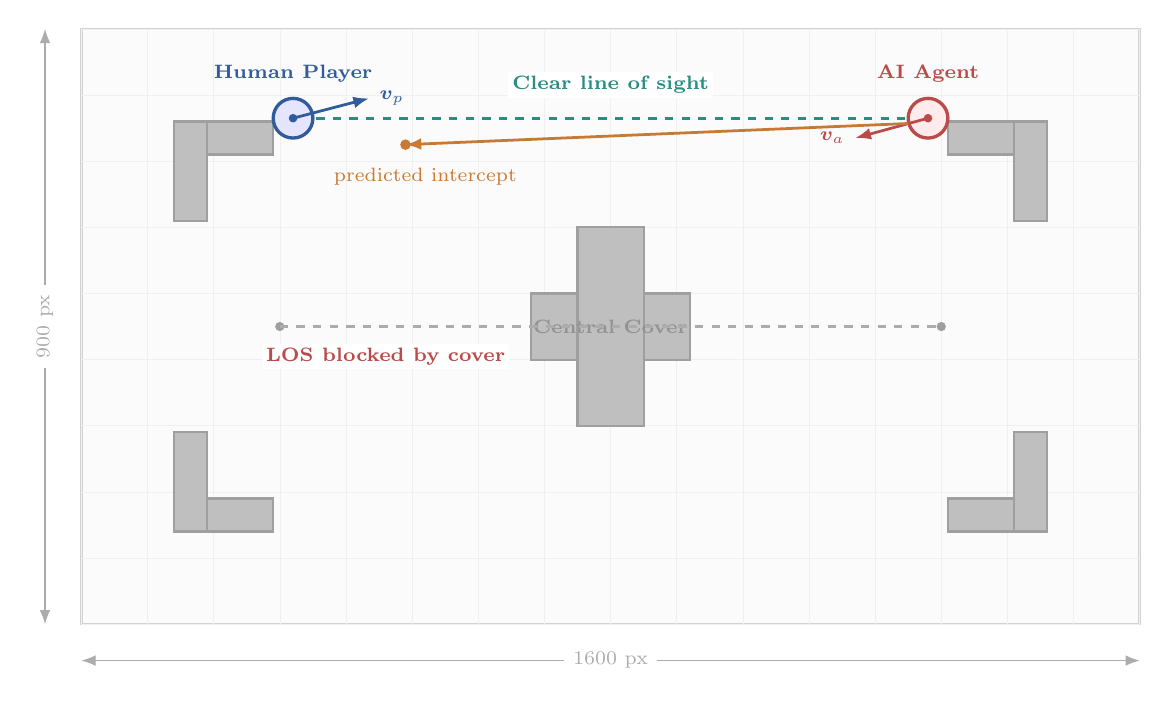
\begin{tikzpicture}[x=0.84cm,y=0.84cm,font=\small]
        % Arena
        \draw[fill=gray!3,draw=gray!35,line width=0.9pt] (0,0) rectangle (16,9);
        \draw[step=1,gray!12,very thin] (0,0) grid (16,9);

        % Central cross
        \draw[fill=gray!50,draw=gray!75,line width=0.8pt] (6.8,4.0) rectangle (9.2,5.0);
        \draw[fill=gray!50,draw=gray!75,line width=0.8pt] (7.5,3.0) rectangle (8.5,6.0);
        \node[font=\scriptsize\bfseries,text=gray!85] at (8,4.5) {Central Cover};

        % Corner L covers
        \foreach \x/\y/\sx/\sy in {
            1.4/6.1/1/1,
            14.6/6.1/-1/1,
            1.4/2.9/1/-1,
            14.6/2.9/-1/-1
        }{
            \begin{scope}[shift={(\x,\y)},xscale=\sx,yscale=\sy]
                \draw[fill=gray!50,draw=gray!75,line width=0.8pt] (0,0) rectangle (0.5,1.5);
                \draw[fill=gray!50,draw=gray!75,line width=0.8pt] (0.5,1.0) rectangle (1.5,1.5);
            \end{scope}
        }

        % Player and agent, placed high enough to avoid central cover
        \draw[fill=blue!10,draw=paBlue,line width=1.2pt] (3.2,7.65) circle (0.30);
        \fill[paBlue] (3.2,7.65) circle (0.065);
        \node[anchor=south,text=paBlue,font=\scriptsize\bfseries] at (3.2,8.05) {Human Player};

        \draw[fill=red!8,draw=paRed,line width=1.2pt] (12.8,7.65) circle (0.30);
        \fill[paRed] (12.8,7.65) circle (0.065);
        \node[anchor=south,text=paRed,font=\scriptsize\bfseries] at (12.8,8.05) {AI Agent};

        % Velocity vectors
        \draw[-{Latex[length=2mm]},paBlue,line width=1pt] (3.2,7.65) -- (4.35,7.95)
            node[anchor=west,font=\scriptsize] {$\bm v_p$};
        \draw[-{Latex[length=2mm]},paRed,line width=1pt] (12.8,7.65) -- (11.7,7.35)
            node[anchor=east,font=\scriptsize] {$\bm v_a$};

        % Clear LOS
        \draw[paTeal,dashed,line width=1pt] (3.55,7.65) -- (12.45,7.65);
        \node[fill=white,inner sep=1.6pt,text=paTeal,font=\scriptsize\bfseries]
            at (8,8.15) {Clear line of sight};

        % Lead point
        \coordinate (lead) at (4.9,7.25);
        \draw[paOrange,line width=1pt,-{Latex[length=2mm]}] (12.5,7.57) -- (lead);
        \fill[paOrange] (lead) circle (0.08);
        \node[anchor=north,text=paOrange,font=\scriptsize] at (5.2,7.05) {predicted intercept};

        % Blocked LOS example in lower half
        \fill[gray!75] (3.0,4.5) circle (0.07);
        \fill[gray!75] (13.0,4.5) circle (0.07);
        \draw[gray!65,dashed,line width=0.9pt] (3.0,4.5) -- (13.0,4.5);
        \node[fill=white,inner sep=1.5pt,text=paRed,font=\scriptsize\bfseries]
            at (4.6,4.05) {LOS blocked by cover};

        % Dimensions
        \draw[{Latex[length=1.8mm]}-{Latex[length=1.8mm]},gray!65] (0,-0.55) -- (16,-0.55)
            node[midway,fill=white,font=\scriptsize] {1600 px};
        \draw[{Latex[length=1.8mm]}-{Latex[length=1.8mm]},gray!65] (-0.55,0) -- (-0.55,9)
            node[midway,fill=white,rotate=90,font=\scriptsize] {900 px};
    \end{tikzpicture}
    \caption{Arena Cross 地图结构及典型视线/预判射击关系。图中上半部分展示无遮挡情况下的移动目标截击，下半部分展示中央掩体造成的视线阻断。}
    \label{fig:arena_cross}
\end{figure}

\subsection{关键机制及其对智能体设计的影响}
PulseArena 的控制难点并非来自单一动作，而来自多个资源和物理约束之间的耦合。

\begin{enumerate}
    \item \textbf{能量约束射击。}
    射击会消耗 Energy，能量随时间恢复；持续无效开火会削弱后续进攻和防御能力。因此“是否开火”不是单纯的命中率问题，而是带有机会成本的资源分配问题。策略层需要决定射击意图，执行层则应避免明显不可命中的能量浪费。

    \item \textbf{Dash 时机与冷却。}
    Dash 提供短距离爆发位移和短暂防护，但具有约 $2.5$ 秒冷却。若把 Dash 当作普通移动键高频使用，智能体会在真正的高危弹体到来时失去关键防御手段。该机制要求策略显式考虑“当前收益”与“保留技能”的时间权衡。

    \item \textbf{Shield 能量消耗。}
    Shield 能吸收正面射击，但其启动与维持都消耗资源。因此护盾使用应与威胁方向、剩余能量和预期交火时间联合判断，而不是简单地在检测到敌人时持续开启。

    \item \textbf{视线与掩体博弈。}
    障碍物同时影响移动可达性与弹道可达性。角色可以通过 Peek、Strafe 或短时离开掩体获得射击窗口，但暴露时间越长，承受反击的风险越高。由此产生了典型的“探头--射击--回撤”节奏。
\end{enumerate}

从控制角度看，这些机制自然形成两类变量：一类是\textbf{战术上不确定、需要学习的变量}，例如是否主动进攻、选择哪个目标、何时争夺位置；另一类是\textbf{物理上确定或可解析的变量}，例如已知速度下的截击点、已知弹体轨迹下的最近逼近距离。Protocol v2 的核心思想就是针对这两类变量采用不同的求解方式。

% ============================================================
% 3. Architecture
% ============================================================
\section{智能体架构演进：从端到端动作到分层控制}

\subsection{Protocol v1：直接底层控制及其失败模式}
Protocol v1 使用单一策略网络直接将环境观测 $\mathcal{O}_t\in\mathbb{R}^{d}$ 映射到底层动作：
\begin{equation}
    a_t =
    [\Delta x,\Delta y,\theta_{\mathrm{aim}},
    \mathrm{shoot},\mathrm{dash},\mathrm{shield}].
\end{equation}

在约 200M 环境步的训练后，该方案仍存在三个稳定复现的问题。

\begin{itemize}
    \item \textbf{高频动作振荡。}
    相邻时刻策略输出缺少显式的动力学平滑约束，当价值差异较小的多个方向动作交替成为局部最优时，角色会出现左右/前后快速切换。该现象不仅降低可读性，也会因碰撞和惯性造成实际位移效率下降。

    \item \textbf{移动目标瞄准偏差。}
    子弹具有有限飞行速度，因此命中移动目标需要瞄准未来位置而非当前位置。直接策略可以通过大量交互近似学习这种关系，但在本项目中，它往往退化为追踪目标当前坐标，说明网络没有稳定形成可泛化的截击规律。

    \item \textbf{障碍物附近的局部死锁。}
    当期望移动方向与墙面法向冲突时，碰撞系统会截断部分速度分量。策略若持续输出相似方向，便可能在墙角形成重复动作循环。由于奖励通常只在较长时间尺度反映“卡住”的代价，恢复行为难以通过稀疏反馈稳定学习。
\end{itemize}

在该阶段，Protocol v1 对 Scripted Hard 的胜率长期低于 $15\%$。基于上述现象，我们停止继续扩大同一架构的训练规模，并将其作为 \texttt{archive/legacy\_raw\_ai/} 中的历史基线。

\subsection{Protocol v2：分层 Hybrid Tactical Agent}
Protocol v2 将控制链拆分为“策略层”和“执行层”。策略层负责回答\emph{做什么}，执行层负责回答\emph{如何稳定地做到}。整体数据流如图~\ref{fig:protocol_v2_flow} 所示。

\begin{figure}[H]
    \centering
    \resizebox{0.96\textwidth}{!}{%
    \begin{tikzpicture}[font=\small,node distance=0.72cm]
        % top chain
        \node[paEnv] (obs) {游戏环境观测\\\texttt{AgentObservation}};
        \node[paBlock,below=of obs] (builder) {特征与动作掩码构建\\\texttt{TacticalFeatureBuilder}};
        \node[paBlock,below=of builder] (policy) {142 维战术策略网络\\\texttt{Tactical Policy}};
        \node[paEnv,below=of policy] (decision) {四头离散战术意图\\\texttt{HighLevelDecision}};

        % executors
        \node[paExec,below left=1.10cm and 3.55cm of decision] (aim)
            {弹道截击求解\\\texttt{BallisticAimSolver}};
        \node[paExec,below=1.10cm of decision] (threat)
            {弹体威胁分析\\\texttt{ProjectileThreatAnalyzer}};
        \node[paExec,below right=1.10cm and 3.55cm of decision] (fire)
            {射击资源审计\\\texttt{FireControl}};

        \node[paExec,below=1.25cm of threat] (move)
            {移动执行与卡死恢复\\\texttt{MovementExecutor}};
        \node[paBlock,below=0.90cm of move] (arb)
            {动作仲裁与组合\\\texttt{HybridCombatExecutor}};
        \node[paBlock,below=0.72cm of arb] (action)
            {底层物理动作\\\texttt{PlayerAction}};
        \node[paEnv,below=0.72cm of action] (player)
            {游戏物理角色\\\texttt{ArenaPlayer}};

        % arrows
        \draw[paArrow] (obs) -- (builder);
        \draw[paArrow] (builder) -- node[right,font=\scriptsize] {features + masks} (policy);
        \draw[paArrow] (policy) -- (decision);

        \draw[paGuide] (decision.south) |- (aim.north);
        \draw[paGuide] (decision.south) -- (threat.north);
        \draw[paGuide] (decision.south) |- (fire.north);

        \draw[paArrow] (aim.south) |- (arb.west);
        \draw[paArrow] (fire.south) |- (arb.east);
        \draw[paArrow] (threat.south) -- (move.north);
        \draw[paArrow] (move) -- (arb);
        \draw[paArrow] (arb) -- (action);
        \draw[paArrow] (action) -- (player);

        % executor group background
        \begin{scope}[on background layer]
            \node[
                draw=paOrange!80,
                fill=paLightOrange!55,
                dashed,
                rounded corners=5pt,
                fit=(aim)(threat)(fire)(move)(arb),
                inner sep=0.35cm
            ] (execbox) {};
        \end{scope}
        \node[
            anchor=south west,
            font=\scriptsize\bfseries,
            text=paOrange
        ] at ($(execbox.north west)+(0.05,0.08)$)
        {Deterministic execution layer};
    \end{tikzpicture}%
    }
    \caption{Protocol v2 的分层控制拓扑。高层网络只输出战术意图，弹道、威胁分析、资源审计与移动恢复由低层执行器完成，再通过统一仲裁器组合为物理动作。}
    \label{fig:protocol_v2_flow}
\end{figure}

高层策略接收 142 维特征，并通过四个离散动作头输出：
\begin{sloppypar}
\begin{enumerate}
    \item \textbf{Target Slot（7 类）：}
    \textit{NONE, ENEMY\_0, ENEMY\_1, ENEMY\_2, BEST\_VISIBLE, LOWEST\_HEALTH, SCRIPTED}；
    \item \textbf{Movement Mode（12 类）：}
    \textit{HOLD, CHASE, KEEP\_RANGE, STRAFE\_CW, STRAFE\_CCW, RETREAT, SEEK\_COVER, PEEK, SEEK\_PICKUP, MOVE\_CENTER, EVADE, SCRIPTED}；
    \item \textbf{Fire Mode（6 类）：}
    \textit{HOLD\_FIRE, CONSERVATIVE, NORMAL, BURST, ALL\_IN, SCRIPTED}；
    \item \textbf{Skill Mode（6 类）：}
    \textit{NONE, AUTO\_DEFENSE, DASH\_EVADE, DASH\_ENGAGE, SHIELD, SCRIPTED}。
\end{enumerate}
\end{sloppypar}

如果将四个动作头记为 $a_t^{(k)}$，则策略可写成一个条件分解：
\begin{equation}
    \pi(a_t\mid o_t)
    =
    \prod_{k=1}^{4}
    \pi_k\!\left(a_t^{(k)}\mid o_t,m_t^{(k)}\right),
\end{equation}
其中 $m_t^{(k)}$ 表示第 $k$ 个动作头对应的合法动作掩码。该分解降低了单一联合动作空间的组合爆炸，同时保持目标、移动、射击和技能之间通过共享主干特征产生的统计耦合。

\subsection{低层确定性执行器}

\subsubsection{BallisticAimSolver：移动目标截击}
设射手位置为 $\bm s$，目标当前位置为 $\bm p$，目标速度为 $\bm v$，子弹速度标量为 $c$。若假设目标在短时间窗口内近似做匀速运动，则在飞行时间 $t$ 后，目标位置为
\[
\bm p(t)=\bm p+\bm v t.
\]
子弹若要在同一时刻到达该点，必须满足
\begin{equation}
    \left\|\bm p+\bm v t-\bm s\right\|=ct.
\end{equation}

令相对位移 $\bm D=\bm p-\bm s$，两边平方并展开：
\begin{align}
    \|\bm D+\bm v t\|^2 &= c^2t^2,\\
    (\|\bm v\|^2-c^2)t^2
    +2(\bm D\cdot\bm v)t
    +\|\bm D\|^2 &= 0.
\end{align}
定义
\begin{equation}
    a=\|\bm v\|^2-c^2,\qquad
    b=2(\bm D\cdot\bm v),\qquad
    w=\|\bm D\|^2,
\end{equation}
即可得到关于 $t$ 的二次方程
\begin{equation}
    at^2+bt+w=0.
\end{equation}

当 $|a|$ 足够小时，问题退化为一元一次方程；否则计算判别式
\begin{equation}
    \Delta=b^2-4aw.
\end{equation}
若 $\Delta<0$，在当前“目标匀速、子弹匀速”的近似下不存在实数截击时间；若 $\Delta\ge0$，则从两个根中选取最小正根：
\begin{equation}
    t^\star=
    \min\left\{
    t>0\ \middle|\
    t=\frac{-b\pm\sqrt{\Delta}}{2a}
    \right\}.
\end{equation}
最终瞄准点为
\begin{equation}
    \bm P_{\mathrm{aim}}=\bm p+\bm v t^\star.
\end{equation}

这一求解过程的意义在于：网络无需重新从奖励信号中学习“子弹飞行时间导致的提前量”。高层只需判断\emph{是否值得攻击某个目标}，低层即可计算\emph{应朝哪里射击}。实际执行中还需要处理 $a\rightarrow0$、无正根、目标状态切换、最大允许预测时域，以及预测弹道被墙体截断等边界情况。

\subsubsection{FireControl：把“想开火”变成“值得开火”}
FireControl 接收高层 Fire Mode，但并不机械地执行射击，而是进行三类审计：

\begin{itemize}
    \item \textbf{能量审计：}根据当前 Energy、射击模式及预期交火时间决定是否允许持续射击；低能量时对 NORMAL/BURST 进行降级，ALL\_IN 仅用于高价值击杀窗口。
    \item \textbf{弹道可达性审计：}利用 Raycast 检查当前截击方向是否被掩体阻断，避免在不可达目标上浪费资源。
    \item \textbf{多人模式安全审计：}在 2v2 等模式下，根据队友与射线夹角/空间关系抑制明显的友伤风险。
\end{itemize}

因此，Fire Mode 表示的是\emph{战术上的射击偏好}，最终的射击动作则是经过资源与几何约束后的可执行决策。这一分工可以显著减少高层策略需要同时学习的硬约束数量。

\subsubsection{ProjectileThreatAnalyzer：TCA/DCA 风险预测}
对于运动中的敌方子弹，单纯依据“当前距离”进行闪避并不可靠：一颗距离较近但正在远离的子弹不一定危险，而一颗尚远但正在高速逼近的子弹可能需要立即响应。

设子弹与角色的相对位置、相对速度分别为
\begin{equation}
    \bm r=\bm x_b-\bm x_r,\qquad
    \bm u=\bm v_b-\bm v_r.
\end{equation}
在短时匀速假设下，相对距离平方为
\begin{equation}
    d^2(t)=\|\bm r+\bm u t\|^2.
\end{equation}
其最小值对应的未截断最近逼近时间为
\begin{equation}
    t_{\mathrm{TCA}}
    =-\frac{\bm r\cdot\bm u}{\|\bm u\|^2}.
\end{equation}
在实际系统中将其限制到预测窗口 $[0,H]$：
\begin{equation}
    \hat t_{\mathrm{TCA}}
    =\operatorname{clip}(t_{\mathrm{TCA}},0,H),
\end{equation}
并计算最近逼近距离
\begin{equation}
    d_{\mathrm{DCA}}
    =\left\|\bm r+\bm u\hat t_{\mathrm{TCA}}\right\|.
\end{equation}

当 $d_{\mathrm{DCA}}$ 小于安全半径且 $\hat t_{\mathrm{TCA}}$ 落入高危时间窗时，系统将当前弹体标记为高风险。此时安全层可以对高层动作进行有限度覆盖，例如优先沿弹道法向移动；若可行空间不足且 Dash 可用，则触发更强的规避动作。这里的关键不是“让 AI 无条件躲开所有子弹”，而是把风险评估转换为一个可解释的连续几何量，为后续难度控制提供接管依据。

\subsubsection{MovementExecutor 与 StuckRecovery}
MovementExecutor 使用滞后与平滑机制抑制相邻决策步之间的方向翻转。对于障碍物附近的卡死问题，StuckRecovery 维护最近 $k$ 个时间步的位置序列
\[
[\bm x_{t-k},\ldots,\bm x_t],
\]
并结合期望位移与实际位移的偏差估计卡死状态。如果策略持续给出非零移动意图，而实际位移在多个时间步内低于阈值，则执行器临时进入恢复状态，依次尝试切向移动、短距离后退与绕障。恢复完成后，控制权重新交还高层策略。

这种设计本质上是一种\textbf{局部控制保护层}：它不决定长期目标，只处理对战术无关、但会破坏动作稳定性的局部动力学异常。

% ============================================================
% 4. Difficulty calibration
% ============================================================
\section{从“Elite 不可玩”到推理侧五档难度校准}

\subsection{高强度策略的可玩性问题}
在 Protocol v2 稳定后，我们使用 8 卡分布式 PPO 与 League 对抗进行长时训练。约 500M 环境步后得到的高强度策略在客观对局中表现优秀，但真人测试暴露出两个典型问题。

\begin{itemize}
    \item \textbf{收益驱动的保守 Camping。}
    当奖励函数对生命值损失较敏感时，策略在取得领先后倾向于优先守住优势。配合低层精确截击和掩体判断，AI 可能长时间停留在 Corner Cover 附近，等待玩家主动进入不利交火区。这种行为从胜率角度合理，却降低了对局节奏。

    \item \textbf{机器级规避精度。}
    TCA/DCA 与确定性执行器能够在非常短的时间尺度上做出一致反应。若安全覆盖层始终以最高灵敏度工作，真人玩家会观察到过度稳定的“最后时刻闪避”，从而产生明显的非人感。
\end{itemize}

这说明训练阶段的“最优策略”与部署阶段的“合适对手”应当解耦。本文因此采用一个主 checkpoint，并在推理阶段对策略分布和安全接管频率进行校准。

\subsection{推理侧三参数控制}

\subsubsection{采样温度 $T$：控制决策确定性}
对于某个离散动作头，设网络输出 logits 为 $\bm z$，则温度采样为
\begin{equation}
    p_i(T)
    =
    \frac{\exp(z_i/T)}
    {\sum_j\exp(z_j/T)}.
\end{equation}
在合法动作集合固定的前提下，较大的 $T$ 会压平动作概率差异，使次优动作更容易被采样；较小的 $T$ 则放大 logit 间差距，使策略更接近贪心选择。因而 $T$ 主要控制\textbf{高层决策的随机性与确定性}，而不是直接修改网络能力。

\subsubsection{动作掩码软化 $S_{\mathrm{soften}}$：控制“无效尝试”概率}
硬动作掩码会把非法或当前不可用动作完全排除。对于高难度 AI，这有利于减少明显错误；但对低难度 AI，如果所有显然不合适的动作都被严格删除，即使提高温度，策略仍然可能显得过于“懂规则”。

为表达软化机制，可将其等效理解为硬掩码分布与全动作软分布之间的混合：
\begin{equation}
    \bm p_{\mathrm{mix}}
    =
    (1-S_{\mathrm{soften}})\bm p_{\mathrm{hard}}
    +
    S_{\mathrm{soften}}\bm p_{\mathrm{soft}},
    \qquad
    S_{\mathrm{soften}}\in[0,1].
\end{equation}
其中 $\bm p_{\mathrm{hard}}$ 只在合法动作集合上归一化，而 $\bm p_{\mathrm{soft}}$ 保留被掩码动作的有限概率质量。这样，$S_{\mathrm{soften}}$ 越大，低难度策略越可能出现“时机不对的技能尝试”“缺乏视野时的低价值射击”等次优行为。

需要区分的是：\textbf{软化并不绕过游戏引擎的物理合法性。}例如技能仍在冷却时，即使高层采样到对应意图，底层也只会得到一次无效尝试或安全降级，而不会真正违反技能冷却规则。该机制模拟的是决策失误，而不是修改游戏规则。

\subsubsection{安全兜底阈值 $\theta$：控制确定性系统的接管频率}
对于高层策略输出，可以定义一个置信度统计量 $c_t$（例如所选动作概率或多头聚合置信度）。当
\begin{equation}
    c_t < \theta
\end{equation}
且当前状态同时触发安全/异常条件时，系统允许 Scripted Hard 或确定性安全逻辑接管部分动作。

因此，在当前参数定义下，$\theta$ 越高，满足 $c_t<\theta$ 的状态越多，安全兜底越频繁；$\theta$ 越低，则更多保留神经策略本身的不确定行为。该参数主要控制\textbf{行为可靠性与机器级稳定性}。

\subsection{五档参数配置}
表~\ref{tab:param_config} 给出当前部署使用的五档参数。这里所谓“单调约束”是指三个控制参数随难度呈固定方向变化；\textbf{参数单调并不自动保证胜率严格单调}，因为神经策略与环境动力学是非线性的。最终是否形成强度单调性仍需要通过对局数据验证。

\begin{table}[H]
    \centering
    \caption{PulseArena 推理侧五档难度参数配置}
    \label{tab:param_config}
    \small
    \begin{tabularx}{\textwidth}{lcccY}
        \toprule
        \textbf{难度} &
        \textbf{温度 $T$} &
        \textbf{$S_{\mathrm{soften}}$} &
        \textbf{兜底阈值 $\theta$} &
        \textbf{目标行为特征} \\
        \midrule
        \textbf{Easy} &
        1.60 & 0.30 & 0.55 &
        决策随机性最高，允许更多低价值尝试，安全接管较少，面向新手玩家。 \\
        \textbf{Casual} &
        1.10 & 0.20 & 0.65 &
        具备基本移动与交火能力，但保留较明显的射击和拉扯失误。 \\
        \textbf{Normal} &
        0.85 & 0.10 & 0.75 &
        在稳定战术与可感知失误之间折中，目标是形成“有来有回”的标准体验。 \\
        \textbf{Strong} &
        0.55 & 0.05 & 0.85 &
        决策更接近高概率动作，低层安全逻辑更频繁介入，压迫感明显增强。 \\
        \textbf{Elite} &
        0.25 & 0.00 & 0.95 &
        近贪心决策、严格动作掩码与高频安全兜底，追求最大竞技强度。 \\
        \bottomrule
    \end{tabularx}
\end{table}

三个参数满足
\begin{align}
    T_{\mathrm{Easy}} &> T_{\mathrm{Casual}} > T_{\mathrm{Normal}} > T_{\mathrm{Strong}} > T_{\mathrm{Elite}},\\
    S_{\mathrm{Easy}} &> S_{\mathrm{Casual}} > S_{\mathrm{Normal}} > S_{\mathrm{Strong}} > S_{\mathrm{Elite}},\\
    \theta_{\mathrm{Easy}} &< \theta_{\mathrm{Casual}} < \theta_{\mathrm{Normal}} < \theta_{\mathrm{Strong}} < \theta_{\mathrm{Elite}}.
\end{align}

为避免把不同量纲的原始参数直接画在同一纵轴上，图~\ref{fig:monotonicity} 使用各参数的 min--max 归一化值，仅展示其随难度的\emph{方向性变化}，原始数值仍以表~\ref{tab:param_config} 为准。

\begin{figure}[H]
    \centering
    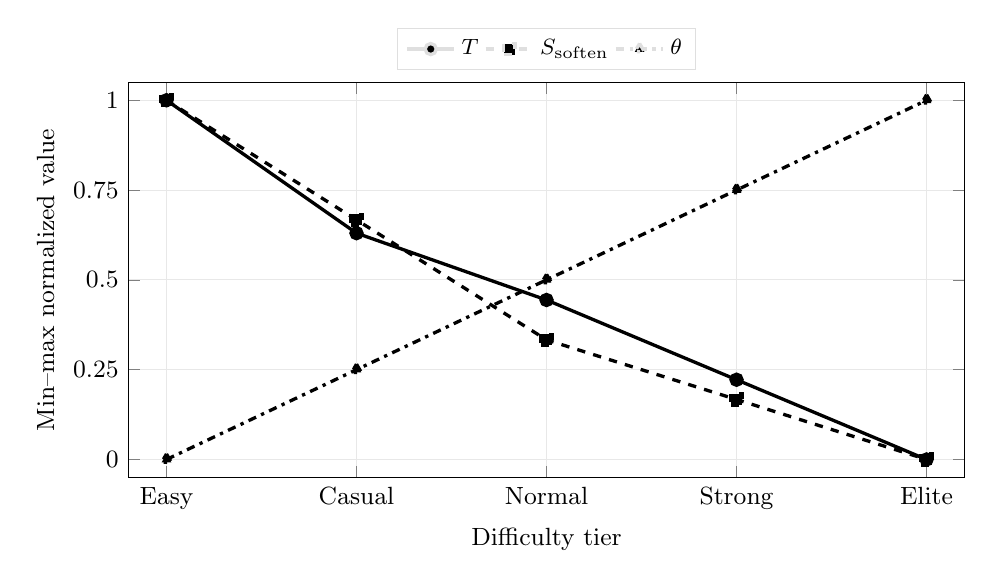
\begin{tikzpicture}
        \begin{axis}[
            xlabel={Difficulty tier},
            ylabel={Min--max normalized value},
            xmin=0.8,xmax=5.2,
            ymin=-0.05,ymax=1.05,
            xtick={1,2,3,4,5},
            xticklabels={Easy,Casual,Normal,Strong,Elite},
            ytick={0,0.25,0.5,0.75,1.0},
            grid=major,
            grid style={draw=gray!18},
            width=12.2cm,
            height=6.6cm,
            legend style={
                at={(0.5,1.03)},
                anchor=south,
                legend columns=3,
                draw=gray!25,
                fill=white,
                font=\footnotesize
            },
            tick label style={font=\small},
            label style={font=\small}
        ]
        \addplot[mark=*,line width=1.2pt] coordinates {
            (1,1.000) (2,0.630) (3,0.444) (4,0.222) (5,0.000)
        };
        \addlegendentry{$T$}

        \addplot[mark=square*,line width=1.2pt,dashed] coordinates {
            (1,1.000) (2,0.667) (3,0.333) (4,0.167) (5,0.000)
        };
        \addlegendentry{$S_{\mathrm{soften}}$}

        \addplot[mark=triangle*,line width=1.2pt,dashdotted] coordinates {
            (1,0.000) (2,0.250) (3,0.500) (4,0.750) (5,1.000)
        };
        \addlegendentry{$\theta$}
        \end{axis}
    \end{tikzpicture}
    \caption{五档推理参数的归一化单调趋势。温度与掩码软化随难度降低，安全兜底阈值随难度升高。该图仅比较变化方向，不表示三类参数具有相同物理量纲。}
    \label{fig:monotonicity}
\end{figure}

% ============================================================
% 5. Implementation and Evaluation
% ============================================================
\section{系统实现与实验评估}

\subsection{Godot--Python 推理链路}
对战引擎运行于 Godot 4.7。Python 训练/推理端与 Godot 游戏端之间通过 WebSocket 中间件 \texttt{serve\_agent.py} 通信。玩家在菜单选择难度后，\texttt{MatchConfig} 将难度写入 \texttt{difficulty}；对局开始后，\texttt{RemoteAgentController} 在每个决策步采集战术特征与动作掩码，并向 Python 服务发送 Protocol v2 请求。

\begin{lstlisting}[caption={Protocol v2 客户端发送给推理服务的战术动作请求示例}]
{
  "cmd": "act_tactical",
  "protocol": 2,
  "request_id": 4012,
  "player_id": 1,
  "model_id": "hybrid_tactical_v1_normal",
  "observation": { ... },
  "tactical_features": [0.12, -0.45, 0.89, ...],
  "action_masks": {
    "target_mask":   [1, 1, 0, 0, 1, 1, 1],
    "movement_mask": [1, 1, 1, 1, 1, 0, 0, 1, 0, 1, 1, 1],
    "fire_mask":     [1, 1, 1, 1, 0, 1],
    "skill_mask":    [1, 1, 1, 0, 1, 1]
  }
}
\end{lstlisting}

服务端根据 \texttt{model\_catalog.json} 中的 manifest 加载同一主 checkpoint，并在 \texttt{sampler.py} 中依据难度应用对应的 $T$、$S_{\mathrm{soften}}$ 和 $\theta$。随后四个动作头完成采样，返回高层战术决策，再由 Godot 侧 HybridCombatExecutor 转换为底层物理动作。

在当前部署环境下，单次 WebSocket 往返时延控制在约 $1.8\,\mathrm{ms}$。该数值是本项目部署条件下的工程测量结果，而非对其他网络环境的通用性能保证。

\subsection{客观胜率单调性}
为验证五档配置是否确实形成可区分的竞技强度，我们使用 Scripted Normal、Scripted Hard 和历史 Baseline v1 作为固定对手，对 Easy--Elite 五档进行了累计约 $10{,}000$ 局离线对局评估。结果见表~\ref{tab:win_rate_results}。

\begin{table}[H]
    \centering
    \caption{五档智能体相对固定基线的客观胜率（报告值及 95\% 置信区间）}
    \label{tab:win_rate_results}
    \small
    \begin{tabularx}{\textwidth}{lcccY}
        \toprule
        \textbf{难度} &
        \textbf{vs Scripted Normal} &
        \textbf{vs Scripted Hard} &
        \textbf{vs Baseline v1} &
        \textbf{观察} \\
        \midrule
        \textbf{Easy} &
        $0.18\pm0.02$ & $0.08\pm0.01$ & $0.12\pm0.01$ &
        对固定基线均处于明显劣势。 \\
        \textbf{Casual} &
        $0.58\pm0.03$ & $0.35\pm0.02$ & $0.48\pm0.02$ &
        相比 Easy 出现显著强度提升。 \\
        \textbf{Normal} &
        $\mathbf{0.78\pm0.02}$ & $\mathbf{0.62\pm0.03}$ & $\mathbf{0.68\pm0.02}$ &
        对规则基线形成稳定优势，同时保留真人对局的可竞争空间。 \\
        \textbf{Strong} &
        $0.92\pm0.01$ & $0.82\pm0.02$ & $0.84\pm0.01$ &
        高压迫档位。 \\
        \textbf{Elite} &
        $0.98\pm0.01$ & $0.93\pm0.01$ & $0.95\pm0.01$ &
        三个基线上均接近压倒性优势。 \\
        \bottomrule
    \end{tabularx}
\end{table}

三个对手上的测得胜率均按照 Easy $\rightarrow$ Elite 的顺序单调上升。这个结果支持“推理侧参数能够有效控制竞技强度”的工程假设，但应注意：\textbf{这是经验上的单调性，而不是由参数顺序直接推导出的数学保证。}如果未来更换 checkpoint、地图分布或奖励函数，仍需重新校准。

\subsection{真人 Human Eval}
真人评测共招募 12 名具有中等射击游戏操作经验的内部测试员，在四张地图上完成累计 610 局对抗。各档实际对局数为 100--150 局，具体分布见表~\ref{tab:human_eval}。评测记录胜负、平均时长、5 分制主观评分，并将评分 $\ge3.5$ 的对局记为“接受”。

在实验前，我们为 Normal 档预先设定体验目标：\textbf{真人对阵 Normal AI 的胜率应位于 $[0.50,0.75]$。}该区间并非普适的人机体验标准，而是 PulseArena 当前内部测试阶段用于描述“玩家有较大胜算、但无法轻松获胜”的工程验收区间。

\begin{table}[H]
    \centering
    \caption{真人对抗评测结果}
    \label{tab:human_eval}
    \small
    \begin{tabularx}{\textwidth}{lccccY}
        \toprule
        \textbf{难度} &
        \textbf{局数} &
        \textbf{真人胜率} &
        \textbf{平均时长 (s)} &
        \textbf{评分 / 5} &
        \textbf{接受率} \\
        \midrule
        \textbf{Easy} &
        120 & $0.92\pm0.02$ & $42.5\pm5.1$ & $3.62\pm0.15$ & $72.5\%$ \\
        \textbf{Casual} &
        120 & $0.78\pm0.03$ & $64.8\pm8.2$ & $3.98\pm0.11$ & $81.2\%$ \\
        \textbf{Normal} &
        \textbf{150} & $\mathbf{0.58\pm0.04}$ & $\mathbf{84.2\pm3.5}$ &
        $\mathbf{4.45\pm0.08}$ & $\mathbf{91.8\%}$ \\
        \textbf{Strong} &
        120 & $0.28\pm0.03$ & $71.1\pm6.8$ & $3.85\pm0.14$ & $78.3\%$ \\
        \textbf{Elite} &
        100 & $0.06\pm0.01$ & $35.4\pm4.2$ & $2.82\pm0.21$ & $35.1\%$ \\
        \bottomrule
    \end{tabularx}
\end{table}

\subsection{结果分析}
\paragraph{Normal 档形成最佳综合体验。}
真人对 Normal 的胜率为 $0.58\pm0.04$，位于预设 $[0.50,0.75]$ 区间内；平均对局时长 $84.2$ 秒，接近 90 秒上限；主观评分与接受率分别达到 $4.45\pm0.08$ 与 $91.8\%$，均为五档最高。结合行为回放，Normal 的 $T=0.85$ 与 $S_{\mathrm{soften}}=0.10$ 使策略仍能稳定执行基本战术，但会出现一定比例的停顿、次优探头和资源使用失误，从而为真人留下反制空间。

\paragraph{Elite 展示了“竞技能力”和“玩家偏好”的分离。}
真人对 Elite 的胜率仅为 $0.06\pm0.01$，平均对局时长下降至 $35.4$ 秒，主观评分为 $2.82\pm0.21$，接受率只有 $35.1\%$。这说明在当前测试群体中，更强并没有带来更高满意度。Elite 仍然有价值，例如作为压力测试、高手挑战或策略上限基线，但并不适合作为默认真人对手。

\paragraph{Easy 也并非越弱越好。}
Easy 下真人胜率高达 $0.92\pm0.02$，虽然对新手具有低门槛优势，但其评分低于 Casual 和 Normal。这提示难度校准的目标不是单调降低 AI 强度，而是让不同玩家群体落在合适的挑战区间。

% ============================================================
% 6. Discussion and limitations
% ============================================================
\section{讨论与局限}

\subsection{为什么 Hybrid 架构适合本项目}
PulseArena 中的核心控制问题具有明显的“可解析/不可解析”分界。弹道截击、最近逼近时间、视线检测等问题具有清晰的几何结构；目标优先级、掩体博弈和何时承担风险则更依赖上下文。让神经网络负责后者、让确定性模块负责前者，能够提高样本效率和调试可解释性。

但 Hybrid 架构也引入了新的风险：低层执行器越强，高层策略越可能依赖这些“隐含能力”；当执行器规则发生变化时，策略分布也可能失配。因此，执行器本身应被视为策略环境的一部分，并在训练、评估和版本管理中保持一致。

\subsection{推理侧难度校准的适用边界}
三参数机制的优点是工程成本低：无需维护五套 checkpoint，也无需为每档重新完成长周期 League PPO。然而它并不能替代真正的多能力策略学习。温度只能改变已有动作概率，无法创造网络从未学习过的战术；掩码软化只能引入更多次优尝试；安全阈值只能改变确定性系统的接管比例。因此，如果需要“新手 AI 会教学”“高手 AI 会诱骗”“某档 AI 具有不同角色风格”等语义层行为，仍需要额外条件化训练或多策略建模。

\subsection{当前实验的限制}
当前结果应被视为项目内验证，而不是对所有竞技游戏的普遍结论，主要限制包括：

\begin{itemize}
    \item \textbf{真人样本量有限。}
    Human Eval 只有 12 名内部测试员，尚未覆盖严格分层的新手、普通玩家和高水平玩家群体。
    \item \textbf{三个推理参数尚未做独立消融。}
    当前五档同时改变 $T$、$S_{\mathrm{soften}}$ 与 $\theta$，因此无法仅从现有结果判断每个参数对胜率与主观体验的独立贡献。
    \item \textbf{策略置信度未必天然校准。}
    神经网络 softmax 概率并不等价于真实正确率，因而基于阈值 $\theta$ 的 fallback 机制可能受置信度失准影响。后续可引入 ECE、可靠性图或单独的置信度校准。
    \item \textbf{固定规则兜底可能被高水平玩家利用。}
    如果 Scripted Hard 的接管逻辑具有稳定模式，长期玩家可能学会识别并针对该模式。
    \item \textbf{当前评估主要集中于胜率与满意度。}
    对“人类感”的评价仍较粗粒度，后续应补充行为多样性、动作熵、掩体驻留比例、反应延迟分布、无效动作率等可解释行为指标。
\end{itemize}

这些限制也给出了下一阶段最直接的实验方向：先进行三参数消融，再扩大真人测试人群，并把“强度”和“行为风格”拆分为两个独立控制维度。

% ============================================================
% 7. Conclusion
% ============================================================
\section{结论与展望}

\subsection{工作总结}
本文围绕 PulseArena 的真人对战智能体设计，完成了从底层端到端控制到分层 Hybrid 控制的架构重构。Protocol v2 将目标选择、移动模式、射击模式与技能模式保留在学习策略中，把弹道截击、威胁几何分析、资源审计和卡死恢复交给确定性执行器。该设计减少了策略网络对低层物理规律的重复学习，并显著提升了控制稳定性。

在此基础上，本文进一步把“训练出强策略”与“部署合适难度”分开处理。通过温度 $T$、动作掩码软化 $S_{\mathrm{soften}}$ 和安全兜底阈值 $\theta$，同一主 checkpoint 被校准为五档强度。离线对局显示三组固定基线上的胜率均随难度单调上升；真人测试则表明，Normal 档在当前测试群体中取得最佳综合体验，而 Elite 档虽然竞争能力最高，却显著降低玩家接受率。

因此，本项目得到的主要工程结论并不是“更弱的 AI 更好”，而是：\textbf{竞技能力与体验难度应作为两个不同问题分别优化。}训练阶段尽可能获得可靠策略，部署阶段再根据玩家目标校准决策确定性、错误概率和安全接管强度，能够以较低维护成本覆盖更广的玩家水平。

\subsection{持续学习闭环}
下一阶段计划构建持续学习闭环：从在线真人对局中收集 replay，经质量筛选后进入 BC/PPO 更新，再对主 checkpoint 和推理侧难度参数重新校准。其流程如图~\ref{fig:feedback_loop} 所示。

\begin{figure}[H]
    \centering
    \begin{tikzpicture}[font=\small]
        \node[paBlock,minimum width=4.2cm] (p1) at (0,0)
            {真人对局\\Human vs Agent};
        \node[paBlock,minimum width=4.2cm] (p2) at (7.0,0)
            {Replay 收集与筛选\\Raw / Curated Replays};
        \node[paBlock,minimum width=4.2cm] (p3) at (7.0,-3.0)
            {BC / PPO 增量训练\\Multi-GPU Training};
        \node[paBlock,minimum width=4.2cm] (p4) at (0,-3.0)
            {难度再校准与部署\\Sampler Auto-Tuning};

        \draw[paArrow] (p1) -- node[above,font=\scriptsize] {record} (p2);
        \draw[paArrow] (p2) -- node[right,font=\scriptsize] {curate} (p3);
        \draw[paArrow] (p3) -- node[below,font=\scriptsize] {checkpoint} (p4);
        \draw[paArrow] (p4) -- node[left,font=\scriptsize] {deploy} (p1);

        \begin{scope}[on background layer]
            \node[
                draw=paTeal!80,
                dashed,
                rounded corners=6pt,
                fit=(p1)(p2)(p3)(p4),
                inner sep=0.45cm
            ] (loopbox) {};
        \end{scope}
        \node[
            anchor=south,
            text=paTeal,
            font=\scriptsize\bfseries
        ] at ($(loopbox.north)+(0,0.12)$)
        {Phase 6: Human-in-the-loop continual improvement};
    \end{tikzpicture}
    \caption{计划中的持续学习闭环。在线 replay 不直接进入训练，而是经过筛选与质量控制后用于 BC/PPO 更新，并在新 checkpoint 上重新进行五档难度校准。}
    \label{fig:feedback_loop}
\end{figure}

未来工作重点包括：（1）对 $T$、$S_{\mathrm{soften}}$ 与 $\theta$ 做严格消融；（2）扩大真人样本并按玩家水平分层；（3）引入行为多样性与“人类感”指标；（4）探索基于玩家实时表现的自适应难度控制，使难度从固定五档进一步发展为连续、个体化的体验校准。

% ============================================================
% References
% ============================================================
\begin{thebibliography}{99}

\bibitem{silver2016alphago}
D. Silver, A. Huang, C. J. Maddison, et al.
\newblock Mastering the game of Go with deep neural networks and tree search.
\newblock \emph{Nature}, 529:484--489, 2016.

\bibitem{vinyals2019alphastar}
O. Vinyals, I. Babuschkin, W. M. Czarnecki, et al.
\newblock Grandmaster level in StarCraft II using multi-agent reinforcement learning.
\newblock \emph{Nature}, 575:350--354, 2019.

\bibitem{schulman2017ppo}
J. Schulman, F. Wolski, P. Dhariwal, A. Radford, and O. Klimov.
\newblock Proximal Policy Optimization Algorithms.
\newblock \emph{arXiv preprint arXiv:1707.06347}, 2017.

\bibitem{nachum2018hiro}
O. Nachum, S. Gu, H. Lee, and S. Levine.
\newblock Data-Efficient Hierarchical Reinforcement Learning.
\newblock In \emph{Advances in Neural Information Processing Systems}, 2018.

\bibitem{csikszentmihalyi1990flow}
M. Csikszentmihalyi.
\newblock \emph{Flow: The Psychology of Optimal Experience}.
\newblock Harper \& Row, 1990.

\bibitem{sutton2018rl}
R. S. Sutton and A. G. Barto.
\newblock \emph{Reinforcement Learning: An Introduction}, 2nd ed.
\newblock MIT Press, 2018.

\end{thebibliography}

\end{document}
